\documentclass[12pt]{article}
\usepackage{lingmacros}
\usepackage{tree-dvips}
\usepackage{graphicx}
\usepackage{color}
\begin{document}

\section{Heap Buffer overflow}

\subsection{Protection which matters}
\begin{itemize}
\item memory randomize 
\item stack guard
\item no excutable stack (optional)
\item malloc check
\end{itemize}
MALLOC CHECK = \\
0 Silently ignore any issue \\
1 Send error message to stderr \\
2 abort() is called immediately, killing your program. \\
3 Do both 1 and 2\\\\ 
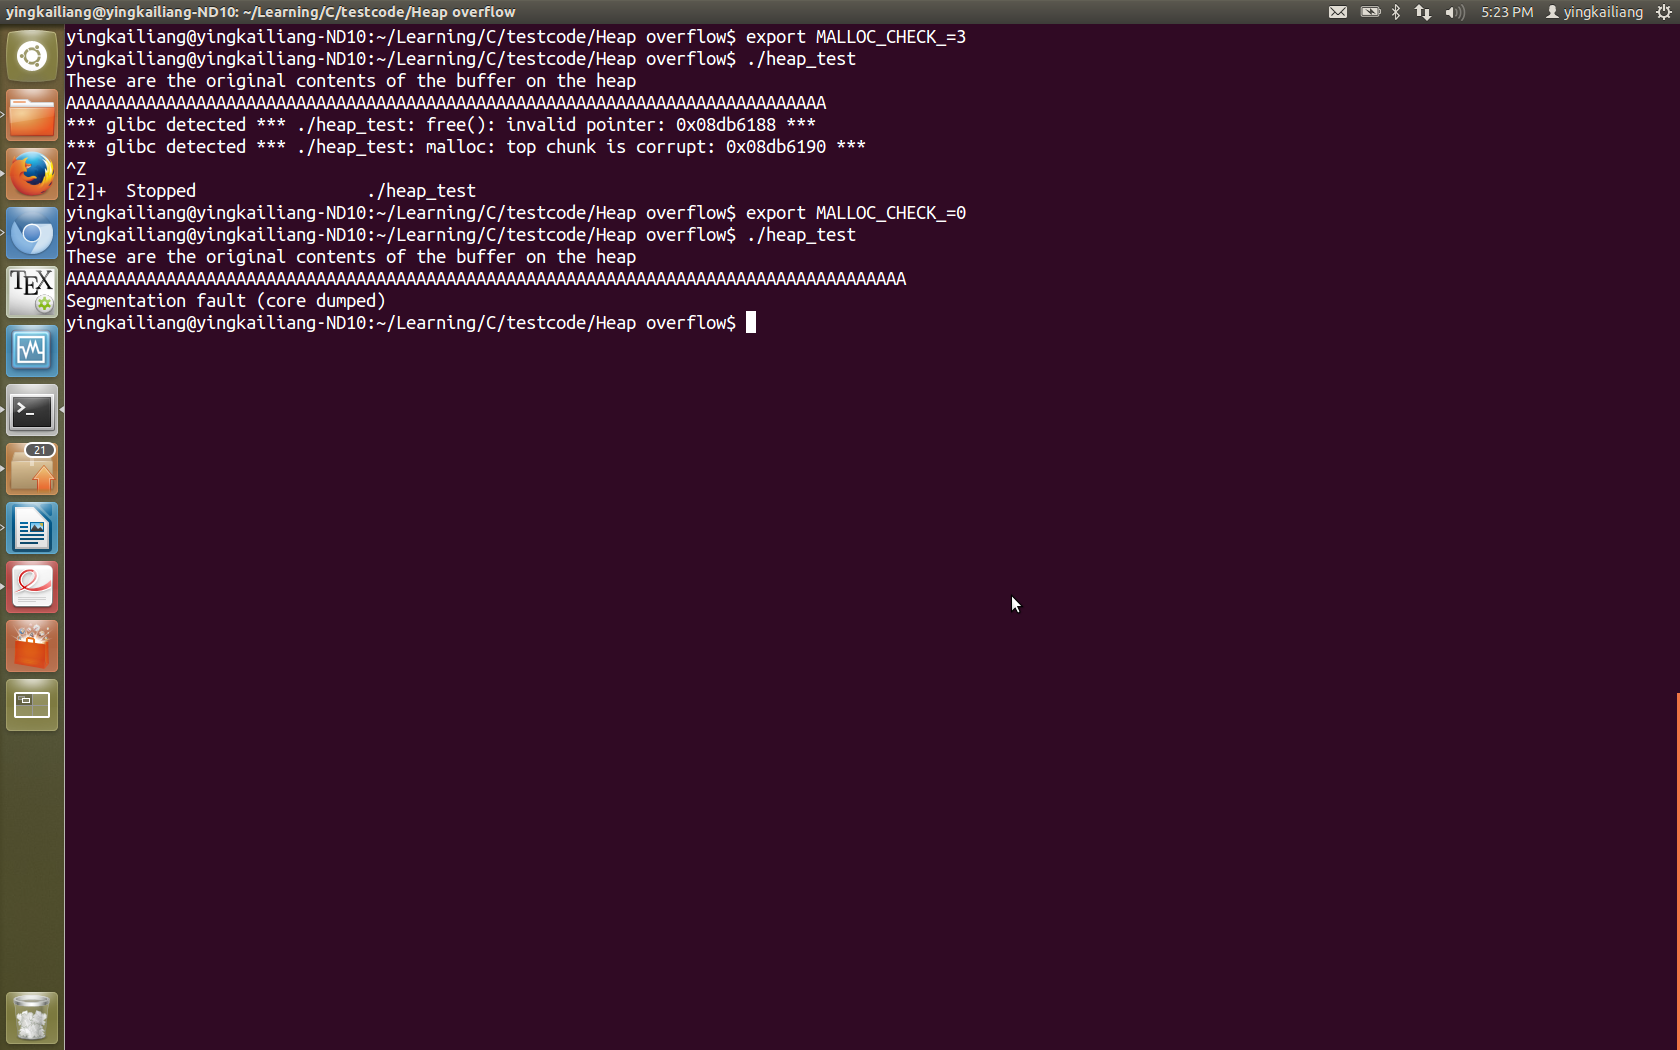
\includegraphics[scale=0.2]{Malloc_check.png} \\

\subsection{Heap layout}

First let's introduce the basic unit data structure used in heap. 

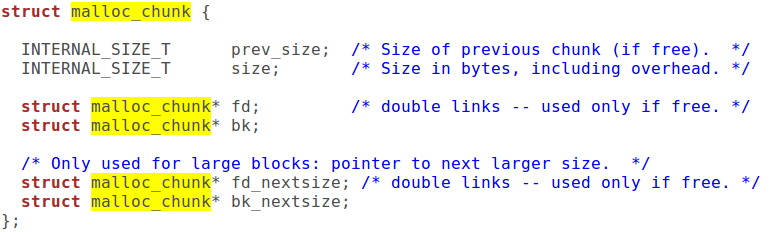
\includegraphics[scale=0.4]{malloc_chunk_code.png}

Malloc\_chunk structure include six fields in it, prev\_size is the size of previous chunk if it is free; size is the current chunk size; fd and fd\_nextsize point to next chunk if it is free; bk and bk\_nextsize point to previous chunk if it is free.   

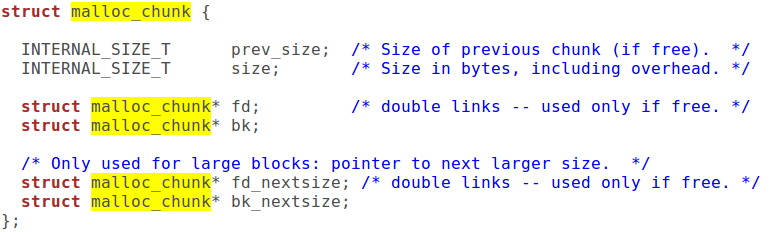
\includegraphics[scale=0.4]{malloc_chunk_code.png}

An allocated chunk in heap look as follow. Two variable store in the head of chunk. The size of previous chunk, if allocated. If not, size will be 0. The second is current chunk size in bytes. Chunk head also contain flags. PREV\_INUSE is what we are interested in. It says whether previous chunk is in used or not. We will use this flag in our latter hypothetical attack. In next chunk is the beginning of the next contiguous chunk.  
 
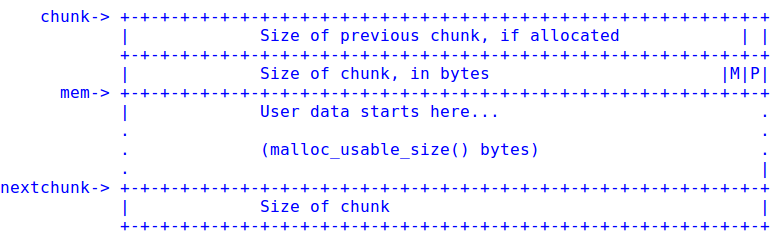
\includegraphics[scale=0.5]{allocated_chunk.png}

A free chunk looks as follow. Free chunks are stored in circular doubly linked lists. Free chunk add two pointers into data field than allocated chunk. One is forward pointer to next free chunk in list. Another is back pointer to previous free chunk in list. As introduce in Malloc\_chunk structure,these two pointer may use fd and bk if chunk is small size. Or may use fd\_nextsize and bk\_nextsize if chunk is large size. 

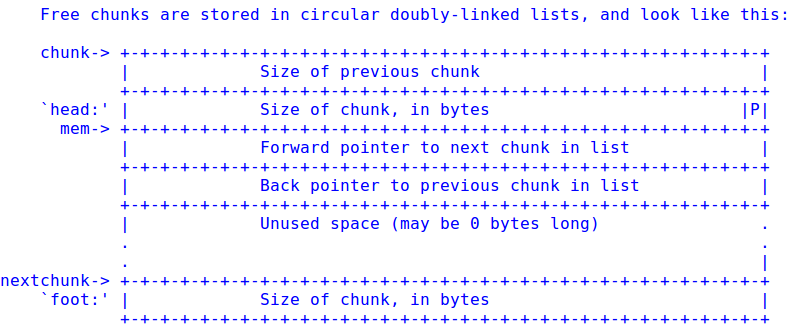
\includegraphics[scale=0.5]{free_chunk.png}

Unlink() function is the function truly free chunk from heap and add to free linked list.Unlink() is in \_int\_free() function. \_int\_free() do all the jobs for free(). The unlink() function assigns forward pointer and back pointer into free chunk.

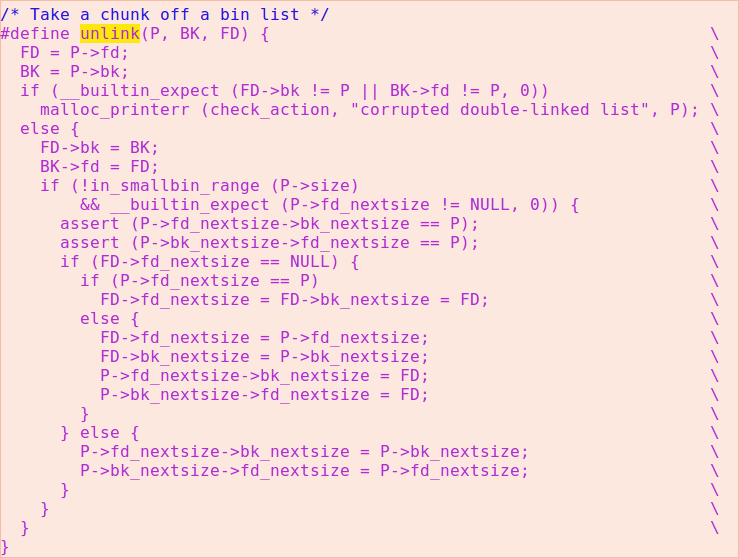
\includegraphics[scale=0.5]{unlink.png}

There are protections in unlink() function to check whether current free chunk is a double-freed-chunk. Double freed chunk is a chunk which be freed twice. This is glibc do not want to happen. 

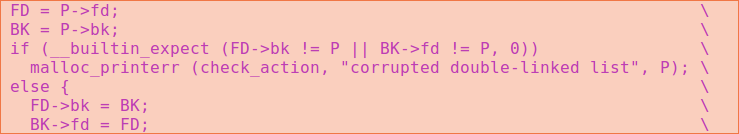
\includegraphics[scale=0.5]{unlink_double_free_check1.png}

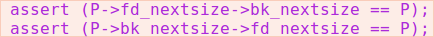
\includegraphics[scale=0.5]{unlink_double_free_check2.png}

After passing all checks, these two line of code will truly remove chunk from linked list if chunk is not in small bin range.   

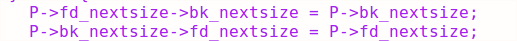
\includegraphics[scale=0.5]{rm_linklist.png}

\subsection{hypothetical attack}

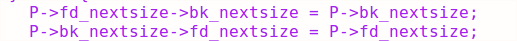
\includegraphics[scale=0.5]{rm_linklist.png}

This equation looks similiar from the old heap overflow address jump equation:\\$p->next->next->pre = p->next->pre$. 

So our hypothetical attack was designed to exploit the same vulnerability in current glibc library. Let $P->fd\_nextsize->bk\_nextsize =$ return address and $P->bk\_nextsize=$ shell code. The hypothetical attack details are as follow.   

The idea is based on glibc malloc.c source code free() function. This is one segment of code inside \_int\_free() function which realize the functionality of free() function. \\
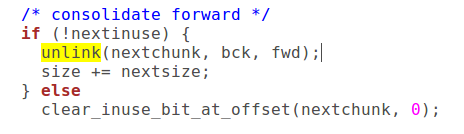
\includegraphics[scale=0.5]{unlink_next_free_chunk.png}

The basic idea is using first buffer to heap overflow the second buffer which both are on heap. After overflow, we intend to create four chunks on heap. Third and fourth chunk are faked chunks created by us. Our third chunk which contains address to shell code on heap and return address to the function frame. The fourth chunk contains shell code and sets the PREV\_INUSE flag to be true in order to fool glibc to think our faked third chunk is an unused chunk and trigger unlink() function to free our third chunk.  

Then the interesting problem becomes how to create these faked chunks. We write our own badfile. When vulnerable program uses system call like fread() to copy data from file to buffer which on the heap, it will overflow the boundary without any boundary checking.

For instance, we assume first heap segment is 12 bytes, this means that glibc expects the size of the second heap segment to start at 13th byte.

I expect to use first segment to overwirte the header of the second heap segment. This is also the heap segment that I am going to free in our vulnerable program. After overflowed, we also want to insert a faked heap chunk which is not inused. As a result of freeing the second heap segment will lead to the execution of our shell code.

In current glibc, there is a fastbin logic which allocates less than 64(0X40) bytes chunkon heap. This is an optimization mechanism holds an array of lists holding recently freed small chunks. Fastbins are not doubly linked. It is single link list. When small chunks less than 64 bytes is allocated. It will first look at fastbin list to find free chunks other than start from the free chunks. 

Fastbin mechanism free chunks differently from unlink() function we see in previous. So the second free chunk has to be bigger than 72(0X48) because 8 bytes aligned in order to avoid triggering fastbin.

Since we've set the previous chunk to be 72 bytes, and the first chunk has 12 bytes of data for us to fill, our 3rd segment will have an 84 byte offset in our copied data.

After bypass error checks which is related to us to access unlink() in \_int\_free()function, we decide our third chunk size is at least 512 byte. So the fourth chunk has offset 84+512 is 596.

At this point we should have made it into the unlink() macro with our faked heap segment passed in as the argument P in unlink(). The first thing unlink() do is set FD and BK to $P->fd$ and $P->bk$. Since we will need to manipulate these values, let's figure out where they are stored exactly on our buffer. The size of badbuffer has an offset 84. we know that the fd and bk fields have offset 88 and 92. We just let fd=bk=0x0804b1c0. Here we use 0x0804b1c0 as example.

Since FD==P, we know that $FD->fd\_nextsize$ is not null, so we only execute the else statement. we want $P->fd\_nextsize->bk\_nextsize$ to be the location on the stack of the return address. We know that the bk\_nextsize field has 20 bytes offset in the malloc\_chunk struct. So we want $P->fd\_nextsize$= return address - 20. In our example the return address is 0xbfffebbc. So minus 20 will be 0xbfffeba8. Our shell code is on 0x804b1e0.   

If all of our assumption succeed, after free the second chunk, heap buffer overflow will be triggered. This is the code to create 4 chunks of segment on heap: \\
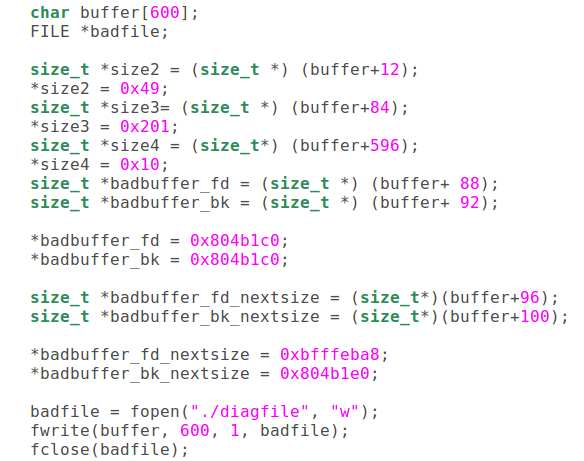
\includegraphics[scale=0.5]{diag_code.png}\\
  
The vulnerable program we provide is:\\ 
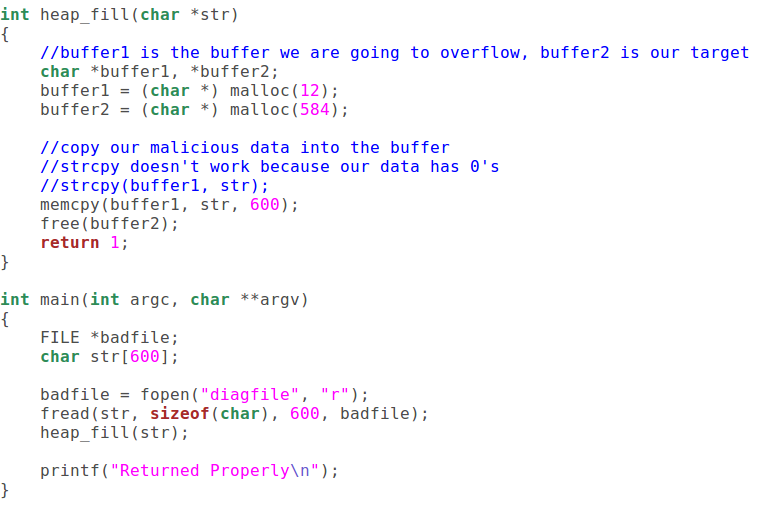
\includegraphics[scale=0.5]{vul_prog.png}\\

The virtual memory layout look at this:\\
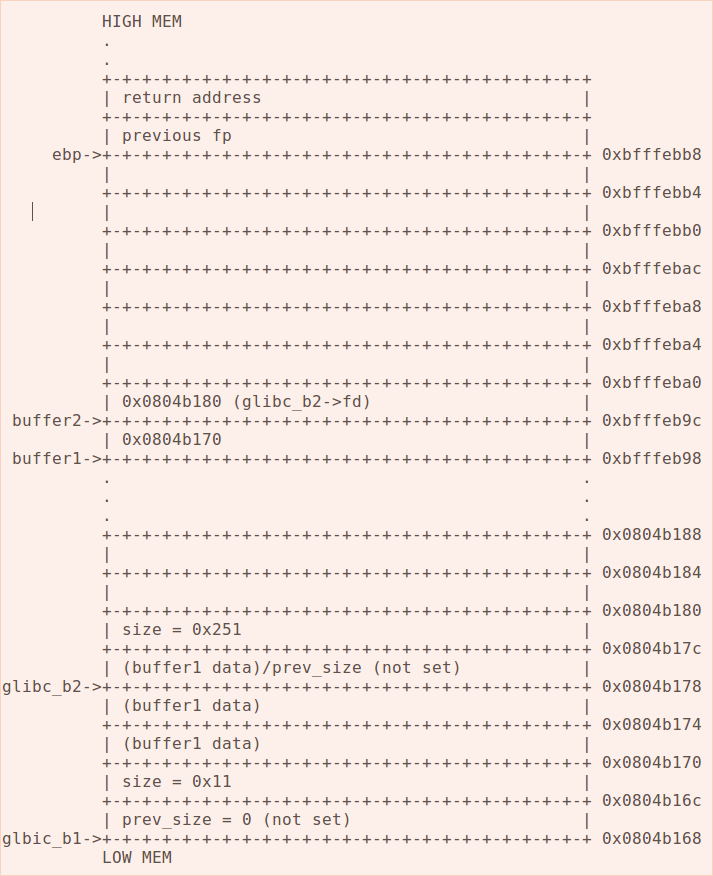
\includegraphics[scale=0.5]{compromised_layout.png}

\subsection{Further Investigation}

Currently, our hypothetic attack is blocked by two assert checks in unlink() function which check whether current freeing block is a double free chunk. Double free chunk means a chunk is freed twiced and appear twice in freed chunk linked list. This situation is not allowed to happen in glibc. This double free check also prevent our attack from happening. 

In order to make our hypothetic attack work, we figure out three options. The first one is try to use flag to turn off these assert checks in unlink function like the protection I introduce in first section. Second approach is that we custmize glibc library by ourself and take out these two assert checks. The third option is that we keep thinking way to bypass these two assert checks.

The first option is the most easy way to achieve the goal. However it depends on whether there exists such a flag or not. The second way takes more time to figure out how to compile glibc for glibc is used for all program. So the difficulty is how to compile glibc and do not let other process running. The third approach is the most hardest way for us right now. For our attack desgin basically, depend on changing one of the pointer value. It is hard to find out an effective way to bypass this assertion check which need all the pointer still point to freed chunk itself. 

\end{document}
